\chapter{Utilisation de TikZ}
\minitoc

Ceci est du text

\section{Figure en traçant avec les coordonnées}

Ceci est du text
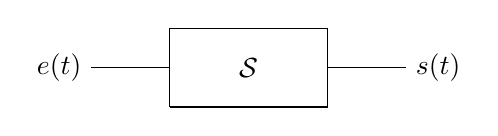
\begin{tikzpicture}
\draw (0,0) -- (2,0) -- (2,1) -- (0,1) -- (0,0); %% on dessine le carré

\draw (-1,0.5) -- (0,0.5); %% le trait horizontal de gauche
\draw (2,0.5) -- (3,0.5); %% celui de droite

%% notations
\draw (-1,0.5) node[left] {$e(t)$};
\draw (3,0.5) node[right] {$s(t)$};
\draw (1,0.5) node {$\mathcal{S}$};


\end{tikzpicture}

\section{Nommage des points}
Ceci est du text

\begin{tikzpicture}
\coordinate (O) at (0,0) ;
\coordinate (A) at (1,0) ;
\coordinate (B) at (0,1) ;
\draw (O) -- (A) ;
\draw (O) node[above,left] {$O$};

\draw (0,0) -- (1,1) arc (180:0:1) -- (4,0);



\end{tikzpicture}

\section{Rectangle}
Ceci est du text

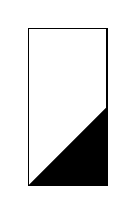
\begin{tikzpicture}
\coordinate (A) at (1,0) ;
\coordinate (B) at (0,2) ;

\draw (A) rectangle (B);
%(0,0) rectangle (2,1);

%\fill (A) rectangle (B);

% like \draw but also fills the shape
\fill (0,0) -- (1,0) -- (1,1) -- cycle;
\end{tikzpicture}


\section{Noeuds}
Ceci est du text

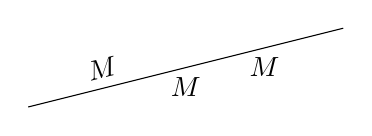
\begin{tikzpicture}
\draw (0,0) -- (4,1) node[midway,below] {$M$}
                     node[near start,above, sloped] {$M$}
                     node[near end,below] {$M$};
\end{tikzpicture}


\section{Coordonnées relatives}
Ceci est du text

\begin{tikzpicture}
\draw (1,2) -- ++(1,1);
\draw (1,2) -- ++(0,2) -- ++ (3,0);
\draw (0,0) -- ++(1,1) -- ++(-1,1) --++ (-1,-1) -- cycle;


\end{tikzpicture}

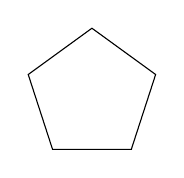
\begin{tikzpicture}
\draw (0,0) -- (1,0)
-- ++(72:1) -- ++(144:1) -- ++(216:1) -- cycle;



\end{tikzpicture}

\section{Décorations, styles, options graphiques}
Ceci est du text
%% colors : red, green, blue, cyan, yellow, magenta, black, white, gray
%% gray!20 gray!40 gray!60 gray!80 gray!100

\begin{tikzpicture}
\draw [very thick, red] (0,0) -- (1,0);
\draw [line width=5pt,green] (0,1) -- (1,1);
\draw [double] (0,2) -- (1,2);
\end{tikzpicture}


\begin{tikzpicture}
\draw [<->] (0,0) -- (1,0) -- (1,1);
\end{tikzpicture}

%\begin{tikzpicture}
%\draw [<->latex] (0,0) -- (1,0) -- (1,1);
%\end{tikzpicture}
%
%\begin{tikzpicture}
%\draw [>=latex,->] (0,0) -- (1,0) -- (1,1);
%\end{tikzpicture}



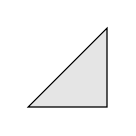
\begin{tikzpicture}
\draw [black,fill=gray!20] (0,0) -- (1,0) -- (1, 1) -- cycle;
\end{tikzpicture}


\section{Axes, grilles, fenêtre d'affichage}
Ceci est du text

\begin{center}
\begin{tikzpicture}
\draw[->] (-1,0) -- (1,0);
\draw (1,0) node[right] {$x$};
\draw [->] (0,-1) -- (0,1);
\draw (0,1) node[above] {$y$};
\end{tikzpicture}
\end{center}


\begin{tikzpicture}
\draw[->] (0,0) -- (4,0);
\draw (4,0) node[right] {$x$};
\draw [->] (0,0) -- (0,4);
\draw (0,4) node[above] {$y$};

\draw [dashed] (2,1) -- (2,0) node[below] {$2$};
\draw [dashed] (2,1) -- (0,1) node[left] {$1$};

\draw [dashed] (0,1.5) -| (1.5,0);
\end{tikzpicture}


\begin{tikzpicture}
\draw [thin, gray, dotted] (0,0) grid (10,8);
\draw (1,0) -- (3,2);
\draw (3,2) node[fill=gray] {$(AB)$};
\end{tikzpicture}

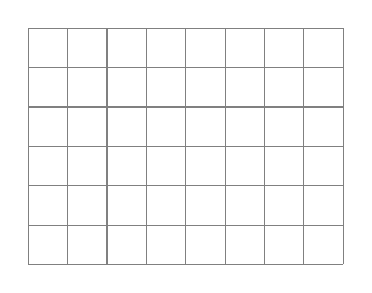
\begin{tikzpicture}
\draw [thin, gray] (0,0) grid[step=0.5] (4,3);
\end{tikzpicture}

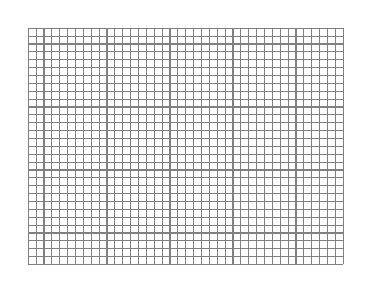
\begin{tikzpicture}
\draw [thin, gray] (0,0) grid[step=0.1] (4,3);
\end{tikzpicture}


\section{Fenêtre d’affichage : clip}
Ceci est du text



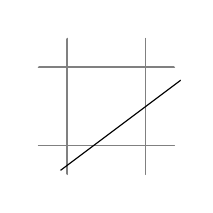
\begin{tikzpicture}
\clip (1.5,1.5) circle (1); %% a mettre en premier
\draw [thin, gray] (0,0) grid[step=1] (4,3);
\draw (0,0) -- (4,3);
%\clip (1.5,1.5) rectangle (2,2);

\end{tikzpicture}



\section{Représentations 3D}
Ceci est du text
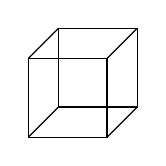
\begin{tikzpicture}
\draw (0,0,0)--(1,0,0)--(1,1,0)--(0,1,0)--cycle; % face arrière
\draw (0,0,1)--(1,0,1)--(1,1,1)--(0,1,1)--cycle; % face avant
% arêtes horizontales, de l’arrière vers l’avant
\draw (0,0,0) -- (0,0,1); % bas gauche
\draw (1,0,0) -- (1,0,1); % bas droit
\draw (1,1,0) -- (1,1,1); % haut droit
\draw (0,1,0) -- (0,1,1); % haut gauche
\end{tikzpicture}



\bigskip

\tikzset{math3d/.style=
{x= {(-0.353cm,-0.353cm)}, z={(0cm,1cm)},y={(1cm,0cm)}}}

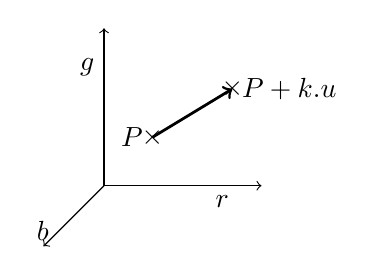
\begin{tikzpicture}[scale=2]
%\draw (0,0) grid (4,4);
\draw[->] (0,0,0) -- ++(1,0,0) node[near end, below] {$r$};
\draw[->] (0,0,0) -- ++(0,1,0) node[near end, left] {$g$};
\draw[->] (0,0,0) -- ++(0,0,1) node[near end, below,left ] {$b$};

\coordinate (P) at (0.5,0.5,0.5);
\coordinate (Q) at (1.2,1,1);

\draw (P) node[left] {$P$};
\draw (Q) node[right] {$P + k.u$};
\draw (P) node {$\times$};
\draw (Q) node {$\times$};

\draw[->, line width=1] (P) -- (Q);

\end{tikzpicture}






\section{Représentation des données}
Ceci est du text

\newcommand{\nombresCopiesParNote}
{(0,0)(1,0)(2,2)(3,0)(4,6)(5,4)(6,7)(7,4)(8,3)(9,0)(10,1)}
\begin{tikzpicture}

\draw plot coordinates {\nombresCopiesParNote};
%\draw plot file {nombresCopiesParNote.txt};
%\draw[thick] plot[xcomb] file {producBle2004.txt}; %% affichage horizontal des données sinon utiliser ycomb

\end{tikzpicture}




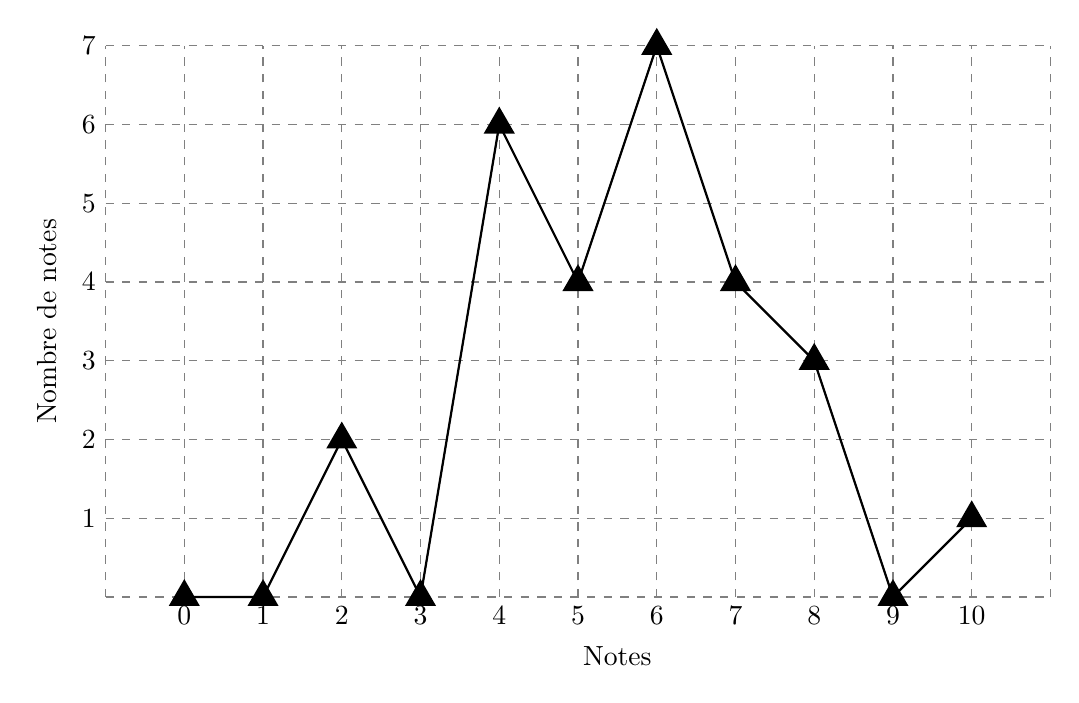
\begin{tikzpicture} % [xscale=0.09,yscale=0.6]
\draw [gray,dashed] (-1,0) grid (11,7);
\foreach \x in {0,1,...,10} \draw (\x,0) node[below]{\x};
\foreach \y in {1,2,...,7} \draw(-1,\y)node[left]{\y};


\draw (5.5,-0.75) node{Notes};
\draw (-1.75,3.5) node[rotate=90]{Nombre de notes};

%\draw[thick] plot[mark=x,mark size=1mm] coordinates {\nombresCopiesParNote}; %% marque les points avec *
%\draw[thick] plot[mark=ball,mark size=1mm] coordinates {\nombresCopiesParNote}; %% marque les points avec *
\draw[thick] plot[mark=triangle*,mark size=2mm] coordinates {\nombresCopiesParNote}; %% marque les points avec *

%% \usetikzlibrary{plotmarks} pour plus de marques différentes

% Tik Z supporte assez mal les points dont les coordonnées sont grandes. L’unité par défaut du dessin est le centimètre. p76 il faut reformater les données

\draw plot coordinates {\nombresCopiesParNote};
\end{tikzpicture}





\section{Graphes}


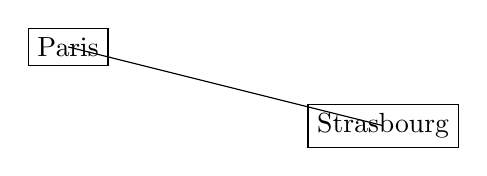
\begin{tikzpicture}

\draw (0,0)node[draw]{Paris} -- (4,-1)node[draw]{Strasbourg};
\end{tikzpicture}



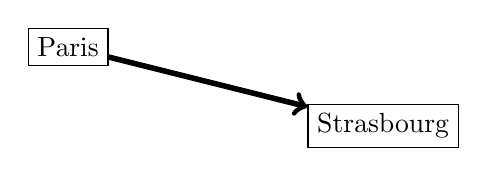
\begin{tikzpicture}
\node[draw] (P) at (0,0) {Paris};
\node[draw] (S) at (4,-1) {Strasbourg};
\draw[->,=>stealth,line width=2] (P) -- (S);
\end{tikzpicture}


\begin{tikzpicture}

\draw (0,0) --(1,1) --(2,0);

\end{tikzpicture}



\begin{tikzpicture}

\node (A) at (1,1) {};
\draw (0,0) --(A) --(2,0);

\end{tikzpicture}



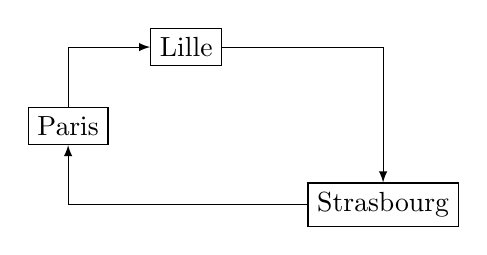
\begin{tikzpicture}
\node[draw] (P) at (0,0) {Paris};
\node[draw] (S) at (4,-1) {Strasbourg};
\node[draw] (L) at (1.5,1) {Lille};

\draw[->,>=latex] (P) |- (L);
\draw[->,>=latex] (L) -| (S);
\draw[->,>=latex] (S) -| (P);
\end{tikzpicture}




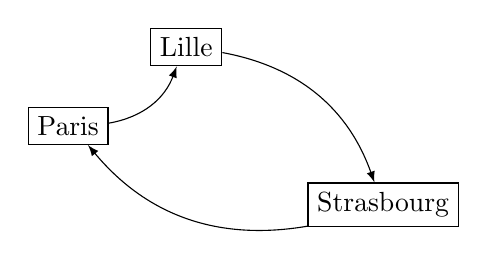
\begin{tikzpicture}
\node[draw] (P) at (0,0) {Paris};
\node[draw] (S) at (4,-1) {Strasbourg};
\node[draw] (L) at (1.5,1) {Lille};

\draw[->,>=latex] (P) to[bend right] (L);
\draw[->,>=latex] (L) to[bend left] (S);
\draw[->,>=latex] (S) to[bend left] (P);


\end{tikzpicture}


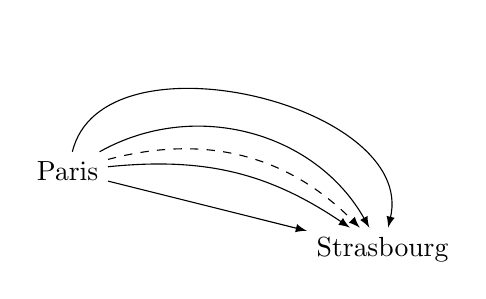
\begin{tikzpicture}
\node (P) at (0,0) {Paris};
\node (S) at (4,-1) {Strasbourg};
%\node (L) at (1.5,1) {Lille};

\draw[->,>=latex] (P) to[bend left=0] (S);
\draw[->,>=latex] (P) to[bend left=20] (S);
\draw[->,>=latex,dashed] (P) to[bend left] (S);
\draw[->,>=latex] (P) to[bend left=45] (S);
\draw[->,>=latex] (P) to[bend left=90] (S);


\end{tikzpicture}


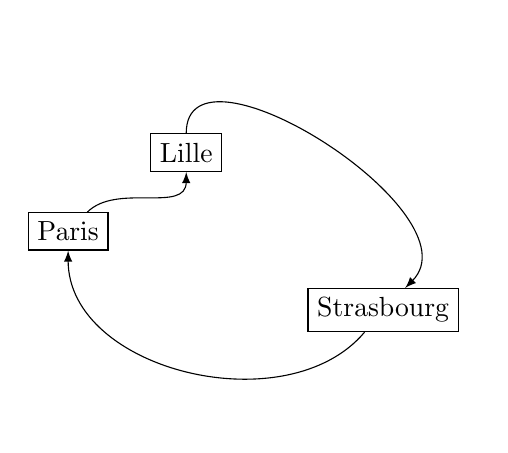
\begin{tikzpicture}
\node[draw] (P) at (0,0) {Paris};
\node[draw] (S) at (4,-1) {Strasbourg};
\node[draw] (L) at (1.5,1) {Lille};

\draw[->,>=latex] (P) to[out=45,in=-90] (L);
\draw[->,>=latex] (L) to[out=90,in=45] (S);
\draw[->,>=latex] (S) to[out=230,in=-90] (P);
\end{tikzpicture}



\begin{tikzpicture}
\draw[{[-]}] (0,0) -- (1,1); \draw[*-o] (2,0) -- (3,1);

\draw[>->>] (4,-2) -- (5,-1); \draw[)-(] (6,-2) -- (7,-1);

\draw[|<-)] (0,-4) -- (1,-3); \draw[{]-)}] (2,-4) -- (3,-3);
\end{tikzpicture}



\section{Frontières des nœuds : circle, ellipse, diamond}




\begin{tikzpicture}

\node[draw,rectangle,rounded corners=3pt] (P)at(0,0){Paris};
\node[draw,minimum height=1cm,dashed] (L)at(2,1) {Lille};
\node[draw,ellipse] (S)at(6,-1) {Strasbourg};
\node[draw,diamond,aspect=2.5] (B)at(0,-1.5) {Bourges};
%% Remarque : L’option diamond est accompagnée de son option aspect qui fixe le rapport entre la largeur et la hauteur du nœud.

\node[draw,circle,fill=gray!50] (D)at(4,-2) {Dijon};

\end{tikzpicture}



\bigskip

\begin{tikzpicture}
%% pgf v1
%\tikzstyle{ville}=[draw,rectangle,rounded corners=3pt]
%\tikzstyle{capitale}=[draw,ellipse,very thick,fill=black!25]

%% pgf v2

\tikzset{ville/.style={draw,rectangle,rounded corners=3pt},
         capitale/.style={draw,ellipse,very thick,fill=black!25},
         radial/.style={very thick,->,>=stealth},
         transversal/.style={<->,>=stealth,thick,dashed}}


%\tikzset{radial/.style={very thick,->,>=stealth’}}
%\tikzset{transversal/.style={<->,>=stealth’,thick,dashed}}

\node[capitale] (P)at(0,0){Paris};
\node[ville] (L)at(2,1) {Lille};
\node[ville] (S)at(6,-1) {Strasbourg};
\node[ville] (B)at(0,-1.5) {Bourges};
\node[ville] (D)at(4,-2) {Dijon};

\draw[radial] (P)--(L);
\draw[transversal] (D)--(B);

\end{tikzpicture}



%% Points d’ancrage des nœuds : N.south, N.left, N.below





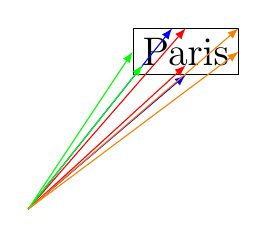
\begin{tikzpicture}
\node[draw] (N) at (2,2) {\Large Paris};
\draw[->,>=latex,red] (0,0) -- (N.north);
\draw[->,>=latex,red] (0,0) -- (N.base);
\draw[->,>=latex,blue] (0,0) -- (N.south);
\draw[->,>=latex,blue] (0,0) -- (N.120); %% N.angle
\draw[->,>=latex,green] (0,0) -- (N.west);
\draw[->,>=latex,green] (0,0) -- (N.text);
\draw[->,>=latex,orange] (0,0) -- (N.east);
\draw[->,>=latex,orange] (0,0) -- (N.north east);
\end{tikzpicture}

